\section{Auswertung}
\label{sec:Auswertung}

\begin{table}[H]
  \centering
  \caption{Messwerte der Wheatstoneschen Brücke.}
  \label{tab:wheat}
  \sisetup{table-format=3.0}
  \begin{tabular}{S[table-format=4.0] S S S[table-format=3.2]}
   \toprule
    {$R_2 $[\si{\ohm}]} & {$R_3$ [\si{\ohm}]} & {$R_4 $[\si{\ohm}]}&{ $R_x = Wert10$[\si{\ohm}]}\\
   \midrule
   332 & 420 & 580 & 240.41 \\
   500 & 325 & 675 &  240.74\\
   1000 & 194 & 806 &  240.70\\
   \bottomrule
  \end{tabular}
\end{table} 

\begin{table}[H]
  \centering
  \caption{Messwerte der Kapazitätsmessbrücke.}
  \label{tab:kap}
  \sisetup{table-format=3.0}
  \begin{tabular}{c S S S S S[table-format=3.2] S[table-format=3.2]}
   \toprule
  &{$C_2$ [\si{\nano\farad}]}&{$R_2$ [\si{\ohm}]} & {$R_3$ [\si{\ohm}]} & {$R_4$ [\si{\ohm}]}&{$R_x$ [\si{\ohm}]} & {$C_x$ [\si{\nano\farad}]}\\
  \midrule
   Wert 9 & 992 & 192 & 691 & 309 & 443.6 & 429.36\\
   Wert 1 & 992 & 0 & 605 & 395 & 647.67 & 0 \\
   \bottomrule
  \end{tabular}
\end{table}

\begin{table}[H]
  \centering
  \caption{Messwerte der Induktivitätsmessbrücke.}
  \label{tab:indu}
  \sisetup{table-format=3.0}
  \begin{tabular}{c S S S S S[table-format=3.2] S[table-format=3.2]}
   \toprule
  &{$L_2$ [\si{\milli\hertz}]}&{$R_2$ [\si{\ohm}]} & {$R_3$ [\si{\ohm}]} & {$R_4$ [\si{\ohm}]}&{$R_x$ [\si{\ohm}]} & {$L_x$ [\si{\milli\hertz}]}\\
  \midrule
  bla
   \bottomrule
  \end{tabular}
\end{table}

Wien-Robinson-Brücke
\begin{figure}
  \centering
  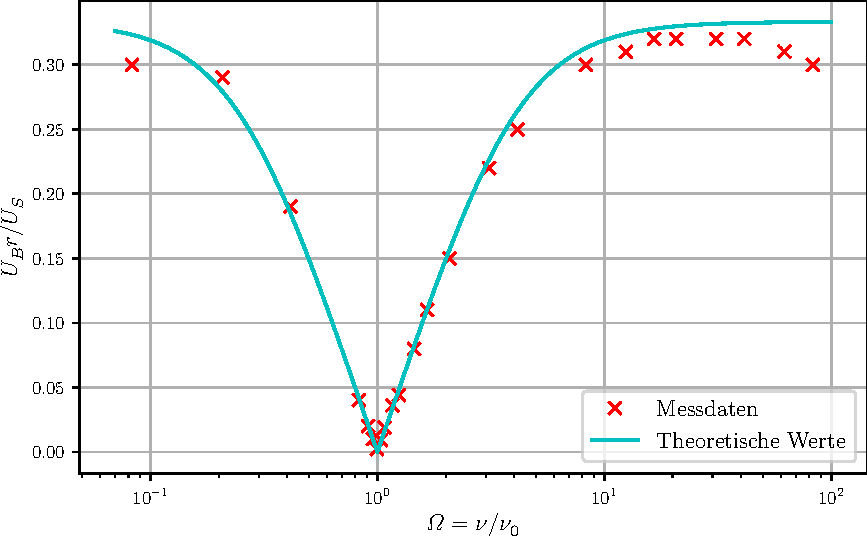
\includegraphics{plot.pdf}
  \caption{keine Ahnung wie man das nennt...}
  \label{fig:wrb-plot}
\end{figure}



